%\hypertarget{estilo:capitulo}{}
%%%%%%%%%%%%%%%%%%%%%%%%%%%%%%%%%%%%%%%%%%%%%%%%%
\section{Materials and method}\label{refmeto}
\subsection{Study Area}
This project admits as a study area the region of S�o Paulo inserted in the hydrographic basin of the River Tamanduate� (Figure \ref{fig:area_estudo}).
This basin has an area of $\SI{323}{\kilo \meter ^2}$ and extends to the hydrographic basins of the Pinheiro, Guai�, Aricanduva and C�rrego de Tapuap� rivers. This area was defined from the vicinity of a rain gauge, according to a spatial radius of \SI{2000}{\meter}, which encompasses different flooding regions, available Tweets and a meteorological radar cell.

\begin{figure}[H]
	\centering
	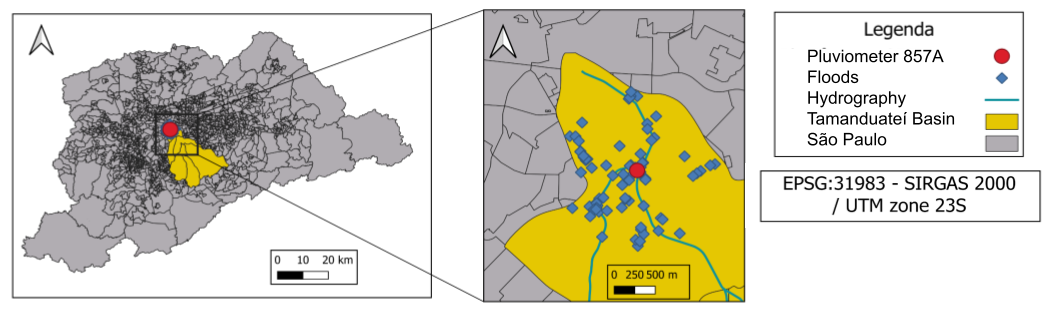
\includegraphics[width=\textwidth]{figs/ic_att2.png}
	\caption{Study Area}
	\label{fig:area_estudo}
\end{figure}

\subsection{Data and tools}
Twitter data were extracted through an API (\textit{Application Programming Interface}) provided by the social network itself. The pluviometric data are collected from the pluviometer $\#833A$, belonging to the National Center for Alerts and Natural Disasters (CEMADEN), which are made publicly available by the institution.
The historical series of flooding in the study area is available through CEMADEN.

The data from the meteorological radar were extracted by a station located in the city of S�o Roque. This equipment, %belongs to CEMADEN and currently
maintained by the Department of Airspace Control (DECEA), it monitors displacement, action of clouds and instability nuclei, measuring the volume of precipitation in a given location. Furthermore, this radar has a range of \SI{250}{\kilo \meter}, covering the entire metropolitan region of S�o Paulo. The radar product used is called CAPPI (\textit{Constant Altitude Plan Position Indicator}),  which has a spatial resolution of approximately \SI{1}{\kilo\meter} and a temporal resolution of 10 minutes. For the conversion of reflectivity (dBZ) into separation rate (mm/h) the Marshall-Palmer ratio \cite{marshall1948mc} will be used, and then represented as ``daily accumulated''.

The development of the project will be guided by programming via the \textit{Python} language. The manipulation, filtering and processing of data will be supported by the \textit{Pandas} \cite{vanderplas2016python} and \textit{Numpy} \cite{mckinney2012python} libraries.

For the application of statistical tests, the \textit{Scipy} \cite{virtanen2020scipy} library will be used. Similarly, the classification methods used in the research (i.e., SVM, RF and MLP) will be obtained from the Scikit-Learn library \cite{pedregosa2011scikit}.

Finally, necessary database operations will be performed with the support of the Geographic Information System \textit{QGIS} \cite{samela2018gis}.

\subsection{Method}

The initial design of this research proposal consists in the use of time series of floods, Tweets, data recorded by rain gauge and meteorological radar, in order to build a method for forecasting flood events.
An overview of the proposal is illustrated in Figure~\ref{fig:metodologia}.

\begin{figure}[H]
	\centering
	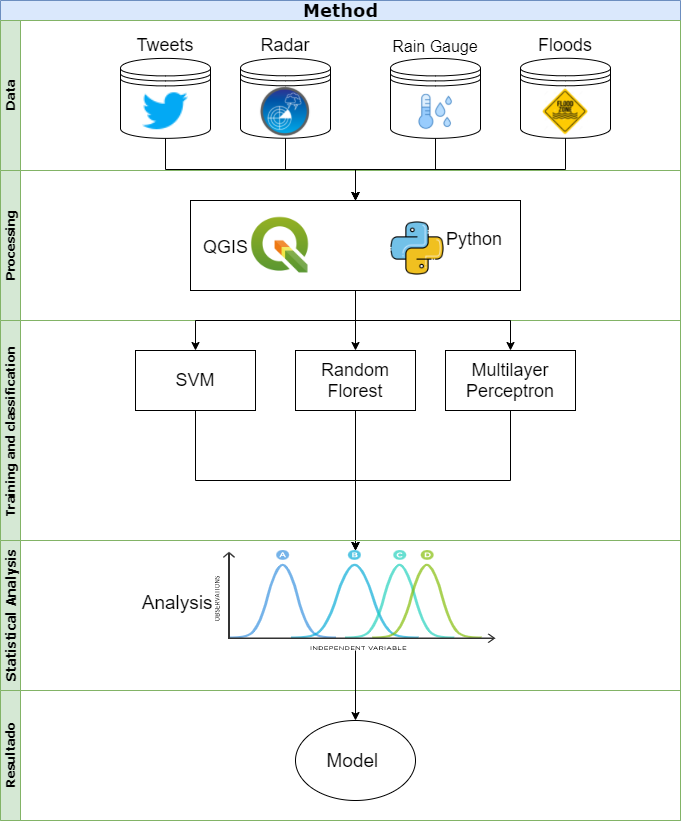
\includegraphics[width=0.6\textwidth]{figs/metodolog.png}
	\caption{Method}
	\label{fig:metodologia}
\end{figure}

Initially, information on the number of filtered Tweets, precipitation values according to radar and rain gauge, and whether there was flooding in the analyzed days will be organized in a single file. In a second moment, this data will be submitted to the SVM, RF and MLP methods. In this phase, different subsets of attributes will be verified among the available ones. An initial division of this base will be admitted, in the proportion $\displaystyle \frac{2}{3} \sim \frac{1}{3}$ for the purposes of training and testing the models. 
The classifications to be carried out will comprise the classes ``flooding'' or ``non-flooding'', whose accuracy will be measured by the basis of tests using measures such as kappa coefficient, F1-Score and cross validation procedure.

Subsequently, statistical tests on the significance of the results will indicate the most relevant method and attributes for building a flood warning system. 